\section{High-Level Overview}
\label{lo:sec:overview}

\begin{figure}[ht]
    \centering
    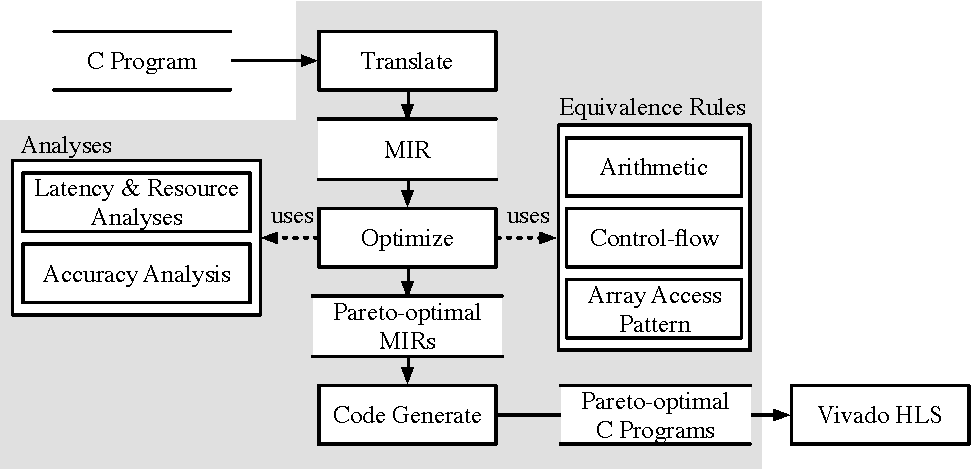
\includegraphics[scale=0.8]{overview}
    \caption{%
        An overview of our automatic program optimization process. The shaded
        region shows our internal tool flow.
    }\label{lo:fig:overview}
\end{figure}

We start by introducing a high-level overview of our program optimization
process (Figure~\ref{lo:fig:overview}).  Our automatic optimization process
starts by taking as an input, the original numerical program written in C, and
translates it into an \gls{mir}\@.  An \gls{mir} is a \gls{dag}, and it serves
as an abstract representation of the original program.  It discards information
about \emph{how} a program is executed, which is dependent on how the program
is structured in C, but retains the \emph{effect} of program execution, keeping
only the structure that leads to the final results.  This procedure, explained
in detail in Section~\ref{lo:sec:intermediate}, greatly reduces the number
of program transformations we need to explore.  We then discover equivalent
\glspl{mir} using our efficient optimization procedure discussed in detail
in Section~\ref{lo:sec:structural_optimization}.  The optimized C programs
can then be generated from the \glspl{mir}, using the \soap{} framework's
code generation routines, to be synthesized in \gls{vhls} to obtain \gls{rtl}
implementations.

As we apply transformation rules to discover equivalent \glspl{mir}, we
estimate latency, resource usage and analyze round-off errors for each
\gls{mir} we have discovered.  Non-Pareto-optimal \glspl{mir}---the ones with
all three performance metrics (latency, resource usage and accuracy) worse
than any other \glspl{mir}---are pruned immediately to keep the size of total
\glspl{mir} discovered tractable.  Section~\ref{lo:sec:performance_analysis}
explains in depth how we analyze latency, resource usage and accuracy.
